\documentclass[book,paper=a4,fontsize=10pt,jafontscale=0.92]{jlreq}

\usepackage{newtxtext,newtxmath}
\usepackage{graphicx}
\usepackage[usenames]{xcolor}
\usepackage{amsmath}
\usepackage{bm}
\usepackage{url}
\usepackage{multirow}

\graphicspath{{./img/}}

% スタイルファイルを1つ選択する(先頭の % を外す) %%%%%%%%%%%%%%%%%%%%%%%%%%%

% 知能・機械工学課程(学部)/知能・機械工学専攻(大学院)
%\usepackage{am-thesis} % 正式提出用
%\usepackage[check]{am-thesis} % チェック用

%人間システム工学科(学部)/人間システム工学専攻(大学院)
\usepackage{hsi-thesis} % 正式提出用
%\usepackage[check]{hsi-thesis} % チェック用

% 以下を適切に設定する %%%%%%%%%%%%%%%%%%%%%%%%%%%%%%%%%%%%%%%%%%%%%%%%%%%%%

% 修士論文/卒業論文の選択

\thesistype{M} % 修士論文はM 卒業論文はB

\title{VRコンテンツ体験時における生体情報に\\基づくリアルタイム感情推定フレームワーク} % あなたの論文のタイトルをここに書く
\author{趙 聖化} % 名字と名前の間は *半角* スペースを入れる．
\studentnumber{27020856} % 8桁で書く．

\syear{2026} % 提出日
\smonth{3}
\sday{1} % 日は出力されない

\mentor{井村 誠孝}{教授} % 指導教員

% 概要 %%%%%%%%%%%%%%%%%%%%%%%%%%%%%%%%%%%%%%%%%%%%%%%%%%%%%%%%%%%%%%%%%%%%%

\abstract{
VR技術の発展に伴い,
ゲームや教育をはじめ様々な分野で没入型のVR(Virtual Reality)体験が普及している.
ユーザに提供される感情的な体験を適切に評価することが求められるが,
従来の評価はアンケートなど主観的手法に依存しており,
リアルタイム性の欠如やバイアスの影響など多くの課題がある.
本研究の目的は,VR体験におけるユーザの感情状態を客観的に評価する方法を探求することである.

本研究では,生体センサと視線追跡を組み合わせた機械学習システムにより,
VR体験中の感情をリアルタイム推定するフレームワークを提案する.
具体的には,皮膚電気活動(EDA),心電図(ECG)から算出される心拍変動(HRV),
筋電図(EMG)などの生体信号と,コントローラ操作ログを同時に収集し,
多角的に解析する.
マルチモーダルな情報を統合して恐怖・驚き・集中などの感情状態を識別することで,
VRコンテンツの感情的効果をリアルタイムに評価可能なシステムを構築する.

(ここはまだ仮説 これから書きます)
提案手法の有効性を検証するため,
Unityを用いたVRホラーコンテンツで被験者実験を行った.
その結果,恐怖刺激に対してEDAが急激に上昇し,
HRV指標の低下やEMG信号の変化が確認された.
また,被験者間で生体反応の大きさに個人差が見られ,
恐怖時に動作が一時停止するいわゆるフリーズ反応も一部で観測された.
得られた知見は,生体・行動情報に基づくリアルタイム感情推定の有効性を示しており,
VR体験の客観的評価手法として本フレームワークが有用である可能性を示唆する.
}

\keywords{
アフェクティブコンピューティング, 生理心理学, マルチモーダルデータ融合
}

% 本体 %%%%%%%%%%%%%%%%%%%%%%%%%%%%%%%%%%%%%%%%%%%%%%%%%%%%%%%%%%%%%%%%%%%%%%%%%%%%%%%%%%

\begin{document}
\pagenumbering{roman}

\jtitlepage % 表紙
\clearpage % 改ページ
\jabstractpage % 内容梗概
\clearpage % 改ページ
\tableofcontents %目次
\clearpage % 改ページ
\listoftables %表目次
\clearpage % 改ページ
\listoffigures %図目次
\clearpage % 改ページ

\chapter{序論}
\pagenumbering{arabic}

VR(Virtual Reality)技術が急速に発展し,
エンターテインメント,教育,医療など様々な分野で没入型のVR体験が提供されるようになっている.
VRコンテンツではユーザに恐怖や興奮,感動といった強い感情的体験を与えることが可能であり,
感情を引き出す効果を高めるための工夫が重ねられている.
一方で,VR体験がユーザに与える感情的影響や体験の質を客観的に評価することは容易ではない.
特に,VRコンテンツ制作者が意図する感情体験がユーザに確実に伝わっているかを検証することは重要な課題であるが,
適切な評価手法は確立されていないのが現状である.

VR体験の効果やユーザの感情反応を評価する際には,
アンケートやインタビューなど体験後の主観評価に頼ることが一般的である.
しかし,主観的な評価には回答者のバイアスや記憶の曖昧さが影響する上,
体験中の瞬間瞬間の感情変化を捉えることはできない.
また,評価のために体験を中断してその場で質問を行うことは没入感の阻害につながるため,
リアルタイムでユーザの感情状態を検出することは困難である.

この問題に対し,工学的アプローチとして,
ユーザの生体信号や行動データを用いて感情状態を客観的に推定する方法が注目されている.
人間の感情は自律神経系の反応として生理指標に現れることが知られており,
例えば皮膚電気活動(Electrodermal Activity; EDA)は交感神経の活動度を反映する指標で,
恐怖や驚きにより覚醒度が高まるとき顕著な上昇を示す.
心電図(Electrocardiogram; ECG)から得られる心拍変動(Heart Rate Variability; HRV)は
副交感神経と交感神経のバランスを示す指標であり,
一般にストレス下ではHRVが低下する傾向が知られている\cite{MarinMorales2020, OrozcoMora2024}.
さらに,筋電図(Electromyography; EMG)は筋肉の活動を測定する手法で,
驚いた際の瞬発的な筋反応や持続的な筋緊張度の変化を捉えることができる.

また,コントローラの操作頻度や動作の変化も感情反応の指標となり得る.
たとえば,突発的な驚き刺激に対して咄嗟に操作が乱れる,
あるいは強い恐怖に直面して一時的に操作が止まる(フリーズ反応)といった現象が考えられる.
以上のように,生体情報と行動情報の双方をマルチモーダルに取得・分析することで,
単一の指標では捉えきれないユーザの内面的な感情変化をより正確に推定できると期待される.

本研究では,このようなアプローチに基づき,
VR体験中のユーザの感情状態をリアルタイムに推定するフレームワークを提案する.
本研究の目的は,生体情報と行動データの統合解析によって
VRコンテンツの感情的効果を客観的に評価する手法を確立することである.
具体的には,EDA,HRV,EMGといった生体センサ情報と,
コントローラの操作ログを同時に取得し,
収集したデータをUnity上のVRコンテンツのイベントと同期させることで,
恐怖・驚き・集中といった感情状態を識別するためのデータセットを構築する.
構築したデータを用いて機械学習モデルを訓練し,
マルチモーダルな特徴量に基づくリアルタイム感情推定を実現することを目指す.

論文の構成をここに書く



\chapter{関連研究}

本章では,本研究に関連する先行研究および基礎知識について述べる.
まず生体信号を用いた感情推定手法について概説し,
次に行動データに基づく注意および感情推定手法を紹介する.
続いて,複数のモダリティを統合するマルチモーダル感情推定の最新動向を考察し,
最後に感情実験の設計およびラベリング手法について説明する.

\section{生体信号に基づく感情推定}

生体信号に基づく感情推定は,
顔表情や音声のような外見的手がかりに依存する手法と比較して,
主観的な操作や偽装が困難であり,
自律神経系および中枢神経系の反応を直接捉えることができるという点で
客観性と再現性に優れている \cite{MarinMorales2020}.

顔表情や音声などの物理的信号は社会的な文脈に応じて意図的に抑制・加工が可能であるが,
心電図,皮膚電気活動,筋電図などは自律神経系によって不随意に制御されるため,
ユーザの本質的な内的状態を高い信頼性で反映する \cite{Shu2018}.   

特にVR環境ではHMDの装着により顔領域の可視性が制限され,
伝統的な表情認識手法の適用が困難であるが,
心電図,皮膚電気活動,筋電図,脳波などの信号は,
ユーザの没入感を阻害することなく同時に収集することが容易である \cite{MarinMorales2020, Liao2020DesignAE}.

収集された生体データは,
VRコンテンツ設計の設計において,どの場面で肯定的あるいは否定的な情動反応が生じたかのを特定する客観的フィードバックや,
ユーザの状態に応じて刺激強度や提示様式を調整する適応型VRの基盤情報として活用できる \cite{MarinMorales2020, OrozcoMora2024}.
ただし,生体信号は感情のみに特異的な信号ではなく,
運動・発話・姿勢変化やVR酔いなどの要因によっても変動するため,
実験設計段階での統制と,アーティファクト除去,ベースライン補正などの信号処理が不可欠である \cite{MarinMorales2020}.

深層学習技術の発展は,生体信号の複雑な非線形パターンの学習に寄与している.
Darらは,14チャンネルEEGの不規則な構造的特性を反映するために,
EEG信号を$81 \times 128$サイズの2次元画像にマッピングして空間的特徴を抽出する2D-CNNアーキテクチャを提案している \cite{Dar2020}.
ECGとGSR信号に対しては,1D-CNNとLSTMを結合して信号の局所的な時間的特徴と長期的な依存関係を同時に学習することで,
感情状態を精密に識別できることを実証している \cite{Dar2020}.

自律神経系指標の中で,心拍変動と皮膚電気活動は情動的覚醒を反映する核心的な指標として広く活用されている.
一般に恐怖のような高覚醒刺激時には交感神経系が活性化し,
心拍数(HR)が上昇し,HRV指標(RMSSDなど)が低下する傾向を示す.
HinkleらはVR環境においてEDA信号のみを用いて高覚醒/低覚醒状態を区別し,
SVMおよびk-NN分類器を通じて最大89\%の認識精度を達成している \cite{Hinkle2019}.

\section{行動データに基づく注意および感情推定}

ユーザの行動ログは生理的反応と密接に関連しており,
注意の集中度や情動状態を間接的に推定する重要な手がかりとなる.
VR環境では,視線追跡,頭部および身体の動き,コントローラ操作ログなどが主要なデータソースとして活用される.
その中でも視線追跡データはHMD内蔵のアイトラッカーを通じて取得可能であり,
注視対象や探索パターンを通じてユーザの関心度や脅威回避行動を分析することに寄与する.

また,コントローラ操作頻度や反応遅延時間などの能動的インタラクションログは,
没入度や恐怖反応を推論するツールとして使用される.
恐怖状況において,ユーザが逃避のために操作を高頻度で行ったり,
逆に極度の恐怖によって身体や操作が一時的に停止する「すくみ(Freeze)」現象が観察されることがある \cite{Pajic2025}.
このようなすくみ反応は脅威に対する人間の本能的な防御機制であり,
VR内でも頭部や手の移動速度が瞬間的に低下する時系列パターンを通じて捕捉可能である \cite{Lin2017}.
行動パターンをイベントのタイムラインと同期させて分析することで,
ユーザの注意の方向と刺激に対する立体的な情動反応を把握することができる.

\section{マルチモーダル感情推定}

マルチモーダル感情推定は,異なる2つ以上のデータソースを結合して対象の状態を推定する方法であり,
感情認識分野でも複数の信号を融合することで性能向上を図る研究が増加している.
単一の生体信号や単一の行動指標だけでは得られる情報に限界があるが,
複数の指標を相互補完的に結合することで,より正確で堅牢な感情分類が可能になる.

生体信号を用いた感情推定研究は活発に行われており,
複数の生体信号を組み合わせることで単一センサーよりも推定精度が向上することが報告されている \cite{MarinMorales2020, Cimtay2020}.
特にVR環境下では,脳波(EEG)と心拍変動(HRV)を用いて感情価と覚醒度を推定する研究 \cite{MarinMorales2018}や,
ユーザの心拍数反応に応じてゲームの難易度をリアルタイムかつ動的に調整する試み \cite{OrozcoMora2024}などがあり,
これは生体情報とコンテンツ間の密接な相互作用である「アフェクティブ・ループ(Affective Loop)」の実現可能性を裏付けている.

このようなマルチモーダルアプローチの優位性は,大規模データセットを用いた実験を通じても証明されている.
Darら(2020)はEEG,ECG,GSR信号を統合し,AMIGOSデータセットで99.0\%,DREAMERデータセットで90.8\%の感情分類精度を達成した \cite{Dar2020}.
この精度は単一モダリティを使用した場合よりも飛躍的に高い数値であり,
異なる生体信号が感情の多様な側面を相互補完的に説明していることを示唆している \cite{Dar2020}.

Arslanら(2024)は,ECGとGSR信号に統計的特徴選択手法を結合して97.78\%の高い精度を記録した \cite{Arslan2024}.
彼らは興奮,幸福,不安,平穏,悲しみの5つの感情状態を分類したが,一部の感情間の境界が曖昧であり,
新規ユーザへの一般化に限界があることも報告している \cite{Arslan2024}.
多くの研究が特定の条件下での感情分類に留まっており,
多様なVR体験や個人ごとの生理的偏差を包括できる汎用的なフレームワークは未だ確立されていないのが実情である.

本研究はこのような限界を克服するため,生体信号(EDA, ECG, EMG)と行動データを統合し,
リアルタイムのイベント同期とベースライン補正を適用した汎用的な感情推定モデルの構築を目指す.

\section{感情実験設計およびラベリング手法}

感情状態を科学的に研究するためには,信頼性の高い感情誘発シナリオの設計と正確な正解ラベル(Ground Truth)の確保が必須である.
VRは従来のメディアよりも強力な没入感を提供し,恐怖や驚きなどの反応を誘発するのに最適化されている \cite{Liao2020DesignAE}.
恐怖研究では,ジャンプスケア要素や照明,音などを活用した環境デザインが主に用いられ \cite{Dozio2022},
Radiahらは,バーチャル環境のレイアウト,色彩,音,装飾,天候という5つの次元のデザイン空間を提案し,
各次元のデザインをリアルタイムで制御してユーザの感情を誘発および評価できる「EmotionEditor」ツールボックスを開発した \cite{Radiah2023}.
このようなツールは実験設計の体系性を高め,研究者が意図した感情状態をより精密に誘導できるようにする.

ラベリング手法は大きく分けて,客観的イベントベースのラベリングと主観的自己報告ラベリングに区別される.
イベントベースの方式は特定の刺激発生時点を基準にラベルを割り当てるためデータ同期が容易である反面,
自己報告方式はSAM(Self-Assessment Manikin)などの尺度を通じて実際のユーザが感じた感情の強度を数値化する \cite{MarinMorales2020, Liao2020DesignAE}.
本研究では主要イベント直後に事後アンケートを実施して獲得した感情強度ラベルを生体データと対照分析することで,
データセットの信頼性を確保する.


\chapter{提案手法}

本研究では,VR環境における没入感を阻害することなく,ユーザの内面的な感情状態を客観的に把握するためのリアルタイム感情推定フレームワークを提案する.本フレームワークは,高精度生体信号センサとVR HMD (Head Mounted Display) の行動ログを統合し,感情状態を多角的に分析する \cite{MarinMorales2020}.

\section{ハードウェアインターフェースおよびセンサ構成}
ユーザの身体反応測定のために以下のようなセンサーを作用する.
\begin{itemize}
\item EMG : 右腕でREF電極を電気的に中立的な骨部位 (bone region) に付着し, IN+およびIN$-$電極を筋繊維方向に整列されるように筋腹 (Muscle belly) の上に20 mm間隔で付着して,筋肉の電気的活動および緊張度を測定する.
\item EDA : 右手のひらに電極を付着し,皮膚伝導度の変化を測定する \cite{Hinkle2019}.
\item ECG : REF電極を腸骨稜 (iliac crest) に付着し, IN+およびIN$-$電極を胸部に付着して,心電図信号を測定する.
\end{itemize}
センサ付着後には電極接触安定化のために必要な手順を遂行した.


\section{生体信号の前処理および数値変換モデル}
BITalinoセンサから収集される生データを物理的意味を持つ単位に変換するため,以下のような変換を行うを適用する.
整体信号取得システムの動作電圧を $V_{CC}$ ,ADC解像度を $n$ ビットとする.

\subsection{心電図 (ECG) および筋電図 (EMG) の変換と前処理}
$$ECG(V) = \left( \frac{ADC}{2^n - 1} - 0.5 \right) \times \frac{V_{CC}}{G_{ECG}}$$
$$EMG(mV) = \left( \frac{ADC}{2^n} - 0.5 \right) \times V_{CC} \times \frac{1000}{G_{EMG}}$$
変換された信号は以下のように前処理される.
\begin{itemize}
\item ECG: 0.5--40 Hz 帯域通過フィルタを適用した後,R-peak検出を実行する.
\item EMG: 20--450 Hz 帯域通過フィルタリング後,整流および包絡線抽出を通じて筋肉緊張度を算出する.
\end{itemize}

\subsection{皮膚電気活動 (EDA) の変換と前処理}
皮膚導電率は、以下の関数を用いてマイクロジーメンス(μS)単位に変換される。
$$EDA(\mu S) = \frac{ADC}{2^n} \times \frac{V_{CC}}{0.132}$$
本公式の分母の $0.132$ は EDA センサーの回路設計に基づく伝達関数の定数である.
EDA信号は0.5 Hz 低域通過フィルタ (LPF) を適用した後,緩やかに変化するSCL (Tonic, トニック) 成分と特定の刺激による急激な変化を表すSCR (Phasic, ファージック) 成分に分解して処理する.

\paragraph{SCL (Skin Conductance Level, Tonic):}
皮膚コンダクタンスの基底レベルを意味する長期的なトニック反応(Tonic level)である. SCLは背景覚醒レベルを反映し, 心理的ストレスや環境的要因によって数十秒から数分にわたって緩やかに変化する特性を持つ. 一般的に一定区間の皮膚コンダクタンス信号の平均または中央値として算出され, 自律神経系緊張度の基底状態を表す指標として活用される.

\paragraph{SCR (Skin Conductance Response, Phasic):}
特定のイベント(Event)や刺激に対する反応として現れる短期的かつ急激な位相性反応(Phasic response)である. 刺激直後約1\textendash5秒以内にコンダクタンスが急激に増加し, 該当刺激に対する神経生理学的覚醒度を直接的に反映する. SCR振幅($SCR_{amp}$)は反応の最大値($SC_{peak}$)と反応開始時点のレベル($SC_{onset}$)の差として定義され, 以下のように算出する.
$$SCR_{amp} = SC_{peak} - SC_{onset}$$



% \section{特徴抽出}
% \begin{itemize}
% \item ECG特徴: 平均心拍数 (HR) および心拍変動指標であるRMSSDを抽出し,自律神経系反応を分析する.
% \item EMG特徴: 筋肉活動の強度を定量化するため,平均電圧,最大電圧,そしてRMS (Root Mean Square) 電圧を算出する.
% \item EDA特徴: 全般的な覚醒レベルを表す平均SCLと,特定刺激による反応回数であるSCRパルス数 (SCR Peaks)を抽出する \cite{Hinkle2019,Shu2018}.
% \end{itemize}
\section{特徴抽出}
前処理された各信号から感情推定に有効な時系列特徴量を抽出する.本研究では,感情状態を反映する生理学的指標として以下の特徴量を算出する \cite{Shu2018}.

\begin{table}[t]
\centering
\caption{抽出された生理学的特徴量の一覧}
\label{tab:features}
\begin{tabular}{llll}
\hline
\textbf{信号} & \textbf{特徴量} & \textbf{単位} & \textbf{生理学的意義} \\
\hline
\multirow{7}{*}{ECG} 
& 心拍数 (HR) & bpm & 全般的な覚醒水準 \\
& RMSSD & ms & 副交感神経活動 \\
& SDNN & ms & 全体的HRV (交感+副交感) \\
& pNN50 & \% & 副交感神経活動比率 \\
& LFパワー & ms$^2$ & 交感+副交感神経活動 \\
& HFパワー & ms$^2$ & 副交感神経活動 \\
& LF/HF比 & - & 自律神経バランス (ストレス指標) \\
\hline
\multirow{3}{*}{EMG} 
& 平均電圧 & $\mu$V & 筋緊張の基礎水準 \\
& 最大電圧 & $\mu$V & 筋活動のピーク強度 \\
& RMS電圧 & $\mu$V & 筋活動エネルギー \\
\hline
\multirow{2}{*}{EDA} 
& 平均SCL & $\mu$S & 基礎的覚醒水準 \\
& SCRパルス数 & 回 & 刺激に対する反応頻度 \\
\hline
\end{tabular}
\end{table}

\subsection{ECG特徴}
心電図から心拍数および心拍変動（HRV）指標を抽出し，自律神経系反応を分析する．

\subsubsection{時間領域HRV指標}
\begin{itemize}
\item 平均心拍数 (HR): 1分間あたりの心拍数（bpm）
\item RMSSD: 連続するRR間隔の差分の二乗平均平方根であり，副交感神経の活動指標として広く用いられる．
\begin{equation}
\mathrm{RMSSD} = \sqrt{\frac{1}{N-1} \sum_{i=1}^{N-1} (RR_{i+1} - RR_i)^2}
\end{equation}
\item SDNN: NN間隔の標準偏差であり，交感・副交感神経の両方を含む全体的なHRV指標である．
\begin{equation}
\mathrm{SDNN} = \sqrt{\frac{1}{N} \sum_{i=1}^{N} (RR_i - \overline{RR})^2}
\end{equation}
\item pNN50: 連続するRR間隔の差が50ms以上である割合（\%）であり，副交感神経活動を反映する．
\end{itemize}

\subsubsection{周波数領域HRV指標}
RR間隔時系列をFFTにより周波数領域に変換し,パワースペクトル密度を算出する \cite{TaskForce1996}．
\begin{itemize}
\item LFパワー (0.04-0.15 Hz): 交感神経と副交感神経の両方の活動を反映
\item HFパワー (0.15-0.40 Hz): 副交感神経活動（呼吸性洞性不整脈）を反映
\item LF/HF比: 自律神経系バランス指標．値が高いほどストレス状態を示す
\begin{equation}
\mathrm{LF/HF} = \frac{\int_{0.04}^{0.15} PSD(f) df}{\int_{0.15}^{0.40} PSD(f) df}
\end{equation}
\end{itemize}

\subsection{EMG特徴}
筋肉活動の強度を定量化するため，以下の特徴量を算出する．
\begin{itemize}
\item 平均電圧，最大電圧 ($\mu$V)
\item RMS電圧: 筋活動の全体的なエネルギー量
\begin{equation}
\mathrm{RMS} = \sqrt{\frac{1}{N} \sum_{i=1}^{N} x_i^2}
\end{equation}
\end{itemize}

\subsection{EDA特徴}
\begin{itemize}
\item 平均SCL ($\mu$S): 基礎的な覚醒水準を示す皮膚電気伝導度の平均値
\item SCRパルス数: 刺激に対する一過性反応の回数 \cite{Hinkle2019}
\end{itemize}

\section{ユーザ入力およびイベントログの活用}
本提案手法では, 生体信号のみならず, VR環境内でのユーザの行動(入力)とシステム側で発生するイベントを統合的に解析することで, 感情推定の精度と解釈性を向上させる.

\subsection{ユーザ入力 (User Input)}
VRコントローラの操作ログとHMDのトラッキングデータを取得し, ユーザの能動的な行動を分析する.
\begin{itemize}
    \item \textbf{トリガー・ボタン入力}: Phase 1での射撃課題(Right Trigger)や, Phase 2での懐中電灯操作(Left Trigger)およびアイテム収集(Ray/Trigger)など, 意図的なインタラクションを記録する.
    \item \textbf{トラッキングデータ (Position/Rotation)}: HMDおよびコントローラの6自由度(6DoF)データを記録する. これにより, 驚き刺激に対する瞬発的な回避動作や, 強い恐怖に直面した際の身体硬直(Freezing)反応などの行動的特徴を抽出することが可能となる. 特にPhase 3では, プレイヤーの視線ベクトルとゾンビの位置関係から「直視(Gaze)」イベントを判定するために活用される.
\end{itemize}

\subsection{システムイベント (System Events)}
VRコンテンツの進行状況や特定の刺激発生タイミングをイベントマーカーとして記録し, 生体信号の文脈(Context)として活用する.
\begin{itemize}
    \item \textbf{フェーズ遷移}: \texttt{PHASE1\_TASK\_START}, \texttt{PHASE3\_START} など, 実験フェーズの切り替わりを記録し, ベースラインとの比較やフェーズごとの状態推定に使用する.
    \item \textbf{タスク・イベント}: Phase 1の試行開始(\texttt{P1\_TRIAL\_ONSET\_GO}), Phase 2のアイテム獲得(\texttt{P2\_PIECE\_n}), Phase 3のゾンビ接近(\texttt{P3\_ZOMBIE\_NEAR\_n})など, 感情変化のトリガーとなる瞬間を特定する.
    \item \textbf{環境変化}: ドアの開閉(\texttt{DOOR\_OPEN})やBGMの切り替えタイミングなどを記録し, 環境要因によるストレス変化を分析する.
\end{itemize}

\subsection{統合解析 (Integration)}
収集された生体信号(EDA, ECG, EMG)とイベントログは, 共通のタイムスタンプおよびサンプルインデックス(\texttt{sample\_index})を用いて厳密に同期される. これにより, 「ゾンビが接近した瞬間」や「アイテムを発見した瞬間」など, 特定の感情生起イベント直後の生理反応(SCRのピーク, 心拍数の急上昇など)をセグメン테ーションし, イベントと生体反応の因果関係を明確にした分析が可能となる.

\chapter{実装}
本章では、提案されたシステムを実際に実装した過程を具体的に記述する.
使用したハードウェアとソフトウェア環境を紹介し,各モジュールの具体的な実装方法を説明する.

\section{開発環境およびシステム構成}
本研究におけるVRコンテンツの実装および実行環境はUnityを基盤としており,HMDにはMeta Quest Proを使用した.
言語およびシステム構成は以下の通りである.
\begin{itemize}
\item Unity側: C\# (VRコンテンツ/イベント発生, TCPクライアント)
\item Python側: TCPサーバ + BITalinoデータ収集/ロギングモジュール
\end{itemize}
Unity (C\#) とPython間の通信はTCPソケット通信で構成し,Unityプロジェクト内の主要通信スクリプトは \texttt{BitalinoController.cs},Python側は \texttt{bitalino\_unity\_server.py} として役割を分離した.


\section{ハードウェア構成}
\subsection{VR HMD: Meta Quest Pro}
本実験では,Meta Quest Proをヘッドマウントディスプレイとして使用した.被験者は両手のコントローラを用いてVR空間内を移動し,特定のインタラクション（ドアの開閉,アイテム取得など）を行うことで,システムへの入力と行動データの収集を行った.

\subsection{BITalinoセンサシステム}
被験者の生理的反応を測定するためにBITalino (r)evolutionボードを使用した.BITalinoデバイスはEMG,ECG,EDAなどのアナログ生体信号を測定し,これを10-bit ADCを通じてデジタル化して出力する.データのサンプリング周波数は1000 Hzに設定した.

収集された各センサのデジタル値は専用センサデータシートに提示された変換公式を通じて物理的単位に換算される.本研究では,前述の提案手法（第3章）で示した数式を用いて各信号の変換処理を行う.具体的なシステムパラメータは以下の通りである.
\begin{itemize}
\item 動作電圧 ($V_{CC}$): 3.3 V
\item ADC解像度 ($n$): 10-bit ($0 \sim 1023$)
\item センサ別ゲイン定数 (Gain): BITalino (r)evolution センサの製造元(PLUX Biosignals)公式データシートに定義された固有値を適用した.
  \begin{itemize}
  \item 心電図 (ECG): $G_{ECG} = 1100$
  \item 筋電図 (EMG): $G_{EMG} = 1009$
  \end{itemize}
\end{itemize}

\subsection{センサチャンネル構成および付着位置}
各センサの付着位置および構成は,第3章(3.2節)で提案した手法に準拠する.具体的なセンサの装着状況を図 \ref{fig:sensor_locations} に示す.

\begin{figure}[t]
  \centering
  \begin{tabular}{ccc}
    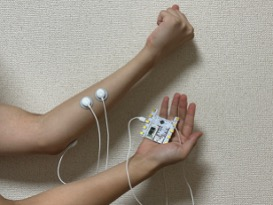
\includegraphics[width=0.3\linewidth]{EMG.jpg} &
    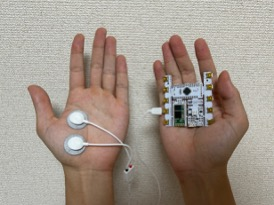
\includegraphics[width=0.3\linewidth]{EDA.jpg} &
    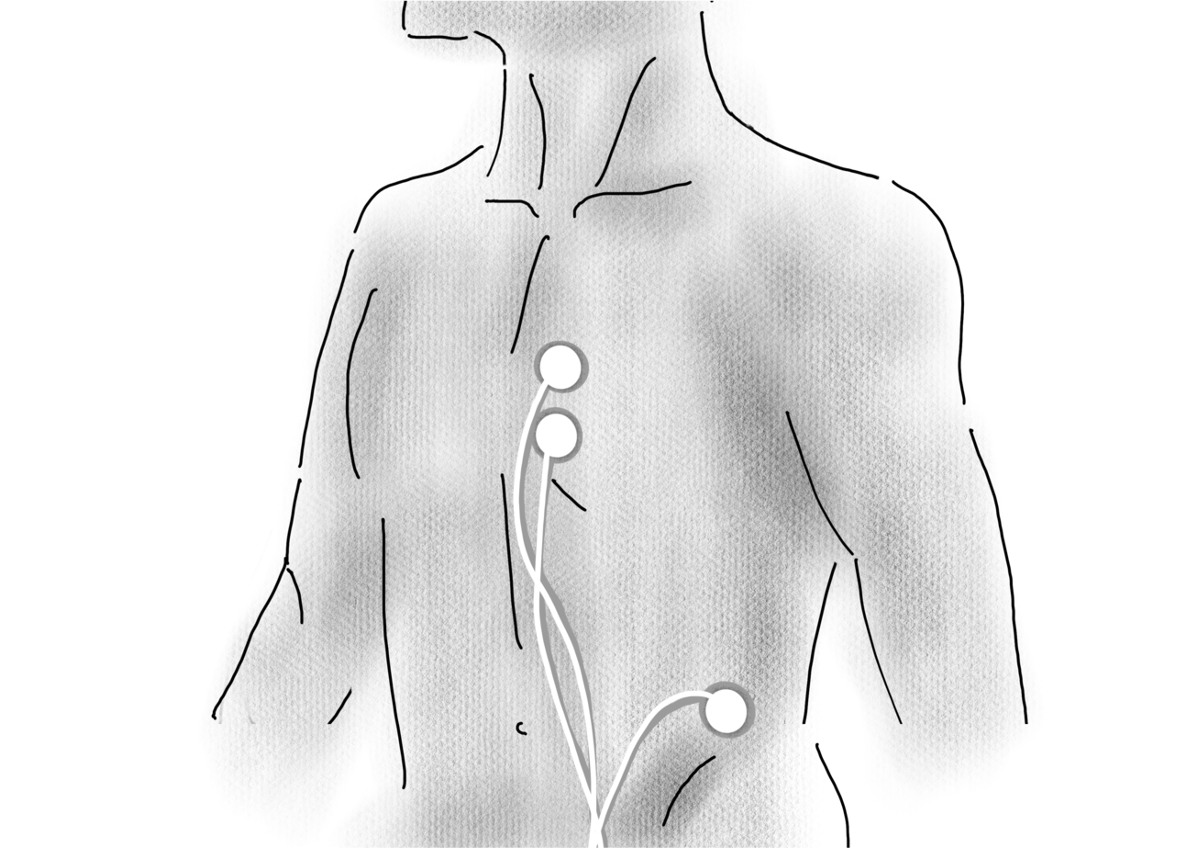
\includegraphics[width=0.3\linewidth]{ECG.png} \\
    (a) EMGセンサ付着位置 (Channel A1) & (b) EDAセンサ付着位置 (Channel A2) & (c) ECGセンサ付着位置 (Channel A3)
  \end{tabular}
  \caption{各生体センサの付着位置}
  \label{fig:sensor_locations}
\end{figure}

\section{ソフトウェア構成}
\section{システムアーキテクチャおよびデータ同期}

本システムは,Unity 2022.3 LTSとPython分析サーバー間の非同期TCP/IPソケット通信を基盤として構築した.各モジュールの役割とデータフローを整理した図を \ref{fig:system_flow} に示す.

\subsection{Unity\textendash Python間TCP同期設計}
本システムの核心は,Unityで発生するイベントタイミングをPythonサーバに伝達し,Pythonが同時に読み取っているBITalinoサンプルストリームと結合(同期)する構造にある.
Unity側では \texttt{BitalinoController.cs}で \texttt{TcpClient} を用いてローカルのPythonサーバに接続し,Phase開始/終了および主要イベント発生時に文字列コマンドを送信する.送信方式は \texttt{writer.WriteLine(cmd)} 形式で改行ベースのメッセージ境界を使用して実装した.
送信コマンドの例は以下の通りである: \texttt{START}, \texttt{STOP}, \texttt{PHASE0\_BASELINE\_START/END}, \texttt{PHASE1\_TASK\_START}, \texttt{P1\_TRIAL\_ONSET\_GO}, \texttt{PHASE2\_SCENE\_START}, \texttt{P2\_PIECE\_1\textasciitilde4}, \texttt{PHASE3\_START}, \texttt{P3\_ZOMBIE\_NEAR\_1/2}, \texttt{P3\_ZOMBIE\_LOOK\_1}, \texttt{DOOR\_OPEN}, \texttt{EXPERIMENT\_END} など.
\texttt{BitalinoController.cs} は実験全体で共通して使用される通信モジュールであるため,シングルトンおよび \texttt{DontDestroyOnLoad} 形式で維持されるように設計し,シーン転換時にも接続状態を保存する.

Python側はTCPサーバとして動作し,Unityから受信したコマンドをイベントログとして記録すると同時に,BITalino装置から生体信号サンプルを持続的に読み取り保存する.特に \texttt{START} 受信時にBITalino接続および測定を開始し,UnityコマンドをイベントCSVとして記録する.

\subsection{イベントログフォーマットと時間同期方式}
イベントログは以下のようなCSVフォーマットで記録する.
\begin{center}
\texttt{unix\_time, sample\_index, label}
\end{center}
ここで \texttt{sample\_index} はBITalino側のサンプルインデックス(または内部カウンタ)で,生理データとUnityイベントを同一時間軸にマッピングする核心キーとして使用する.
Unityイベントは「いつ発生したか」をコマンドで伝達し,Pythonは該当コマンドを受信した時点の \texttt{sample\_index} を共に記録することで,以後の分析段階で生体信号(EDA/ECG/EMG)とイベント(ジャンプスケア/ゾンビ接近/ドア開放など)の整列が可能になる.

\begin{figure}[t]
  \centering
  \fbox{
    \begin{minipage}{0.9\textwidth}
      \centering
      \textbf{System Architecture \& Data Flow} \\[1em]
      \begin{tabular}{c c c}
        \textbf{Unity (VR Client)} & $\xrightarrow{\text{TCP Socket}}$ & \textbf{Python (Analysis Server)} \\
        \fbox{\begin{minipage}{3.5cm}\centering
          VR Environment \\
          (Meta Quest Pro) \\
          \vspace{0.5em}
          Event Triggers \\
          User Input
        \end{minipage}} & & \fbox{\begin{minipage}{3.5cm}\centering
          Data Synchronization \\
          Signal Processing \\
          Feature Extraction
        \end{minipage}} \\
        & & $\downarrow \text{Sync}$ \\
        & & \fbox{\begin{minipage}{3.5cm}\centering
          \textbf{BITalino Sensors} \\
          (ECG, EMG, EDA) \\
          \vspace{0.5em}
          Bio-signals @ 1kHz
        \end{minipage}}
      \end{tabular}
    \end{minipage}
  }
  \caption{提案システムのデータフロー図およびTCP同期メカニズム}
  \label{fig:system_flow}
\end{figure}

\section{Unity側のシステム構成}

Unityプロジェクトでは実験の各Phase（第0相 $\sim$ 第3相）に対応するマネージャスクリプト（例：\texttt{Phase0Manager},\texttt{Phase1Manager},\texttt{Phase23Manager} など）を作成し,イベント発生時の処理を制御した.

\subsection{BitalinoController.csの設計}
Unity環境では \texttt{BitalinoController.cs} が通信の中枢を担う.本スクリプトはシングルトンパターンで実装され,シーン転換が発生しても破棄されない特性を持つ.
\begin{itemize}
\item \textbf{TCP接続確立}: 実験開始時,Pythonサーバへの接続を試みる.
\item \textbf{イベントマーカー送信}: VR空間で発生する全ての意味的イベント(Phase転換,アイテム獲得,敵接近など)を文字列コマンドで構成し,\texttt{writer.WriteLine(cmd)} を通じて即時送信する.ネットワーク遅延を最小化するため,非同期スレッドで処理される.
\end{itemize}

\subsection{コンテンツ設計の基本コンセプト}
本研究で制作したVRコンテンツは,特定の感情状態(集中,恐怖,驚き)を意図的かつ自然に誘発するように設計されたホラーアドベンチャーゲームである.コンテンツはUnityで開発され,暗い屋敷を探索しながらアイテムを収集する「探索型ホラー」形式を採用した.この形式はプレイヤーの自発的行動(探索)と,システム側の予期せぬ介入(ジャンプスケア)を結合することで,多様な感情スペクトルをカバーするのに適している.

\subsection{4段階実験フェーズ構成}
本研究で制作したVRコンテンツは「ランダム迷路型VRホラーゲーム」で構成され, 感情状態を段階的に誘導するためにPhase 0\textendash3の順次構造で設計した.
また, 各フェーズおよびイベントの状況に応じて異なるBGMおよび効果音を使用した. Phase 2の探索パートでは不気味で静かな環境音を再生し緊張感を高め, アイテム獲得時には通知音を鳴らした. Phase 3でゾンビが登場し追跡が始まると, テンポの速い緊迫した追跡用BGMに切り替えることで, 聴覚的刺激による恐怖と焦燥感を増幅させた.
実験は生理信号の変化を正確に測定するため,以下の4つのフェーズに分割して進行する.

\subsubsection{Phase 0: ベースライン (Baseline)}
\begin{itemize}
\item \textbf{目的}: 参加者の安静時生理指標の基準値を確保する.
\item \textbf{環境}: 刺激のない静的な環境で安定した状態で60秒間維持を行い基準(baseline)生理値を確保する(図 \ref{fig:phase0}).
\end{itemize}
\begin{figure}[t]
  \centering
  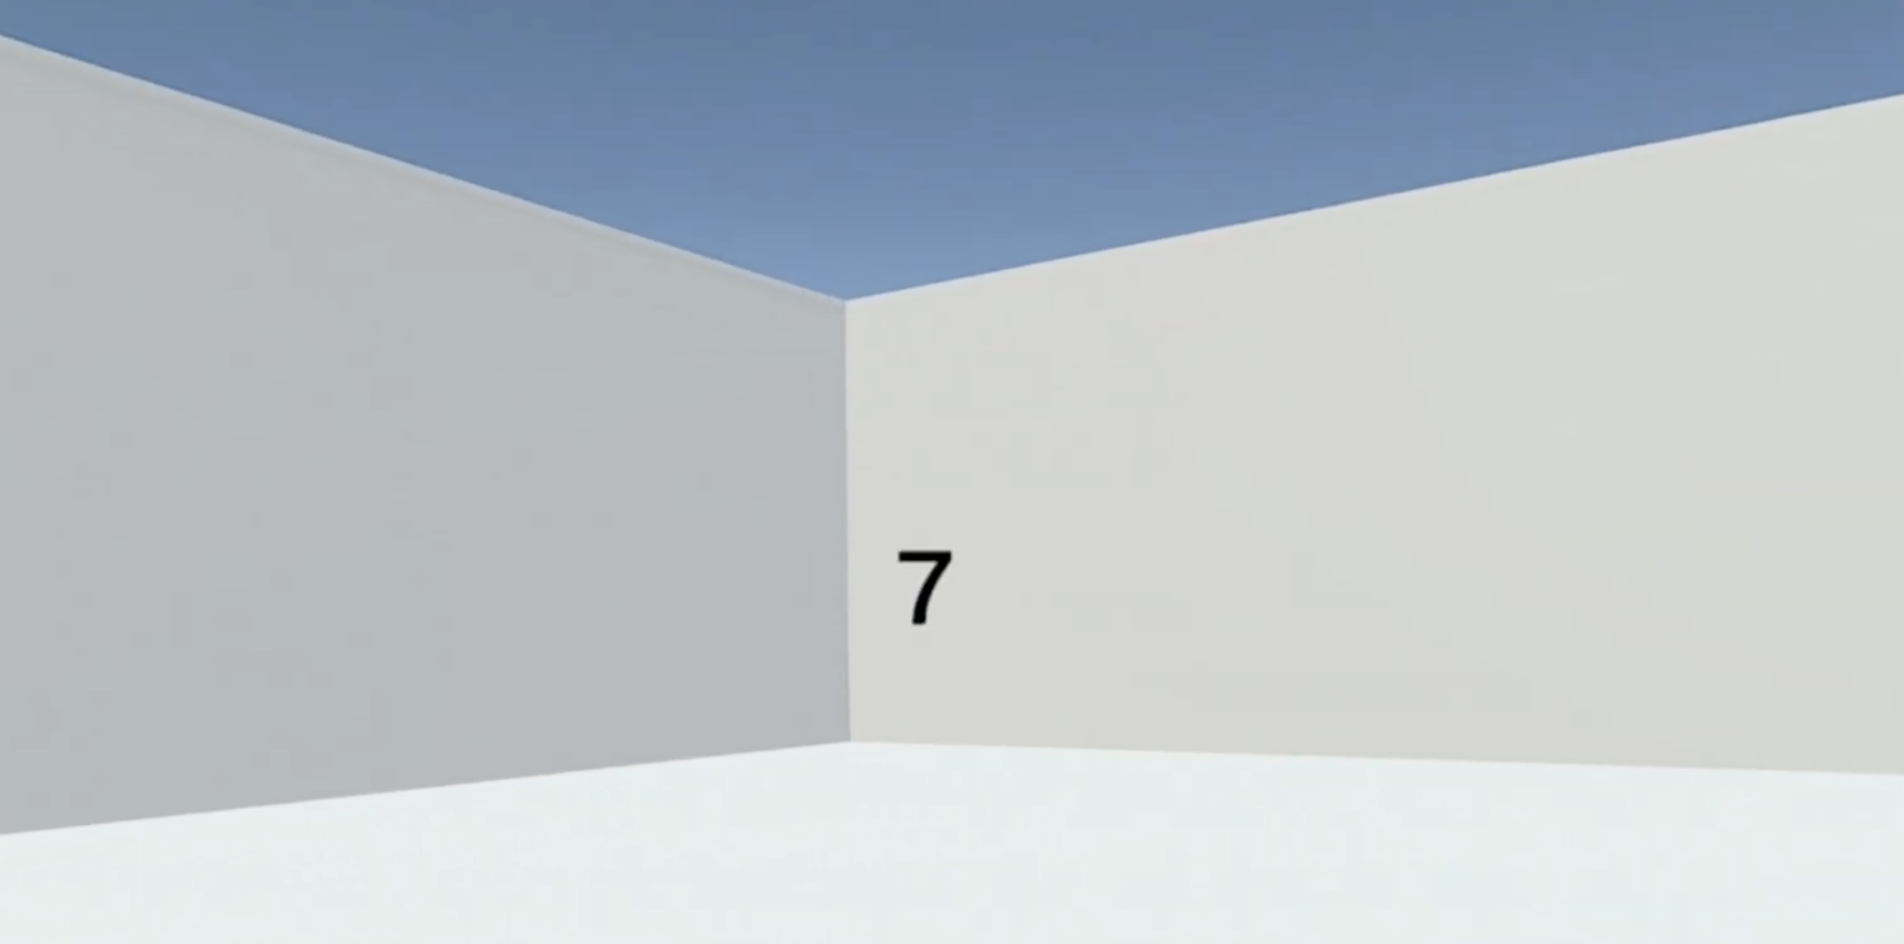
\includegraphics[width=0.6\linewidth]{phase0_baseline.png}
  \caption{Phase 0: ベースライン測定 (安定)}
  \label{fig:phase0}
\end{figure}
この期間のデータは,個人差の大きいEDA・HRVの変化量を正規化するための基準($Baseline$)として使用される.

\subsubsection{Phase 1: 集中課題 (Focus / Go/No-Go Task)}
\begin{itemize}
\item \textbf{目的}: 恐怖・驚きの影響がない状態で「純粋集中」状態の生理データを取得する.
\item \textbf{環境}: 明るいラボ(実験室)風のトレーニングルーム.
\item \textbf{メカニズム}: 恐怖要素を排除した反応抑制課題(Go/No-Go)を遂行させる. 正面に現れる緑の球体(Go)には射撃(トリガー)反応,赤の球体(No-Go)には反応しない抑制課題(図 \ref{fig:phase1}).約30回の試行がランダム間隔で繰り返される.
\item \textbf{ラベリング}: \texttt{P1\_TRIAL\_ONSET\_GO} などのマーカーで課題遂行中の認知負荷と集中状態を記録する.
\end{itemize}

\begin{figure}[t]
  \centering
  \begin{tabular}{cc}
    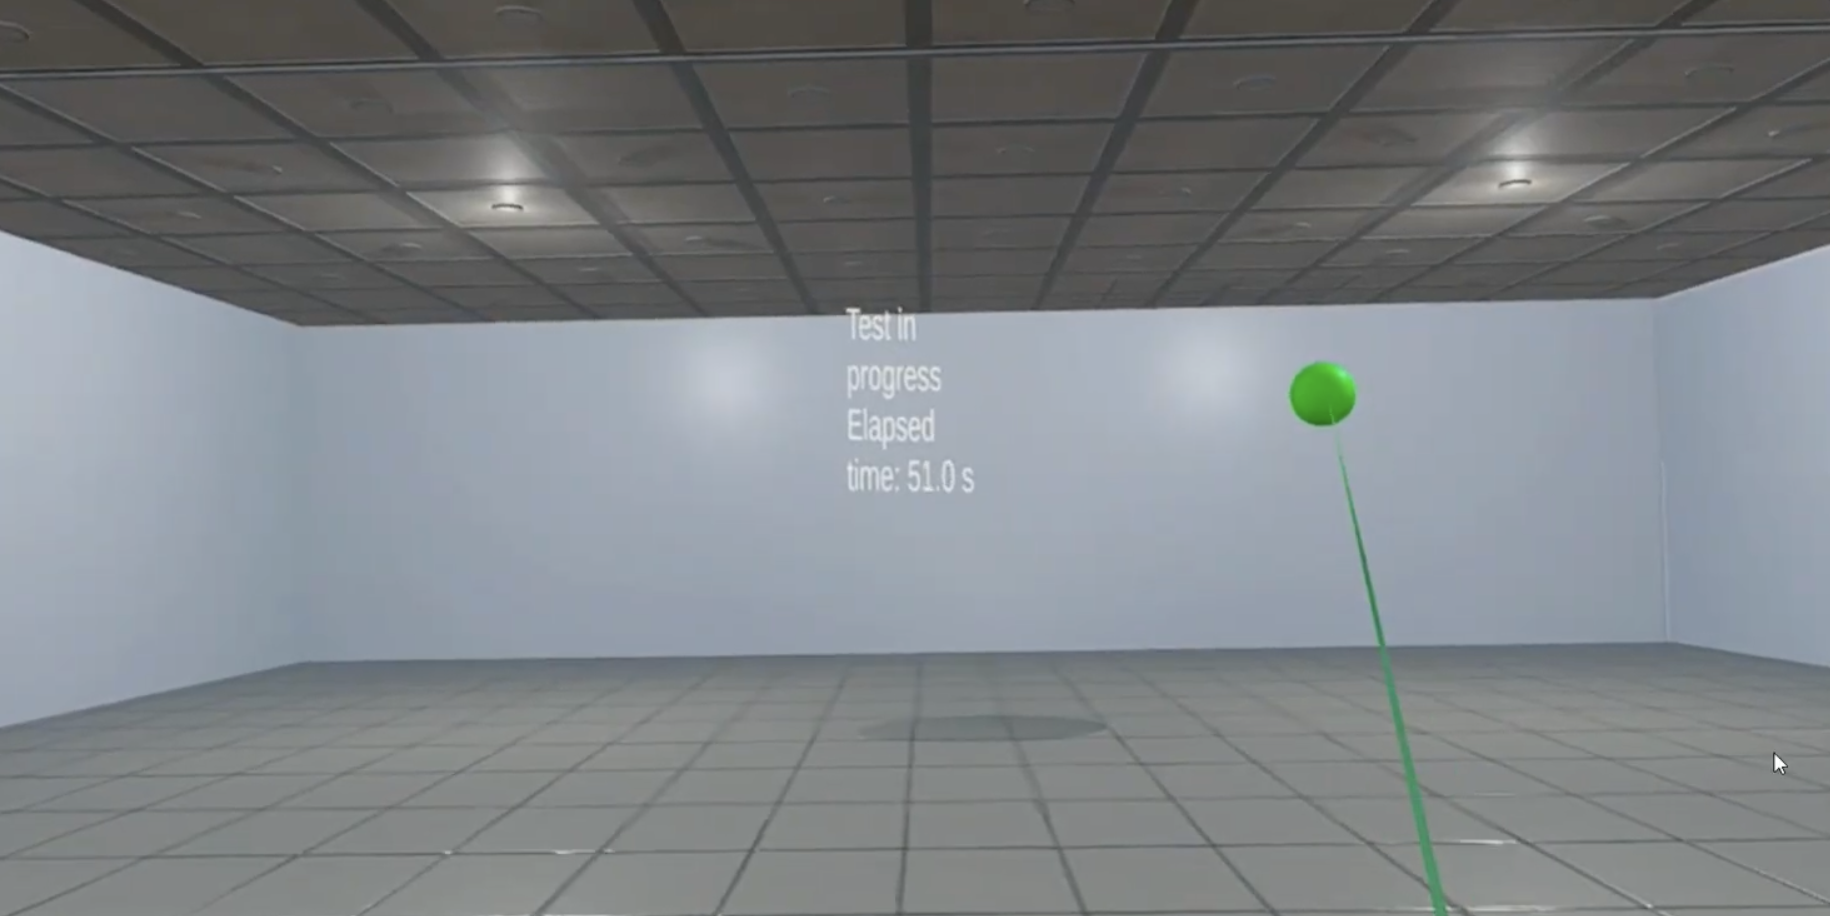
\includegraphics[width=0.45\linewidth]{phase1_go.png} &
    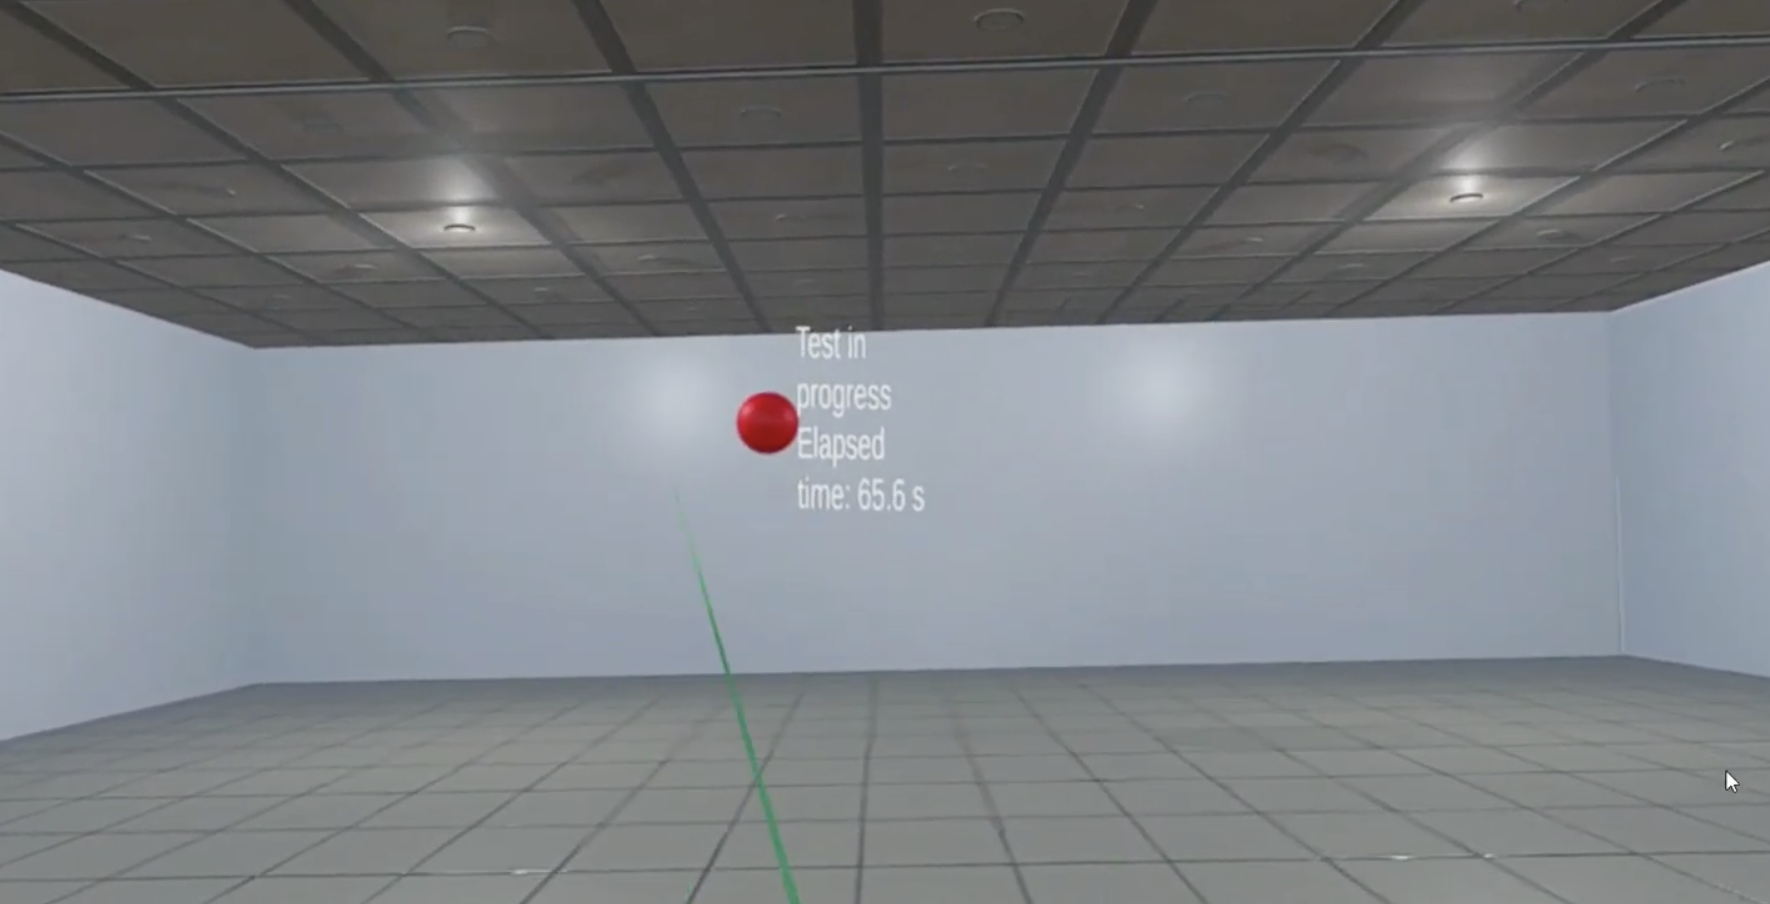
\includegraphics[width=0.45\linewidth]{phase1_nogo.png} \\
    (a) Go課題 (緑のボール・射撃) & (b) No-Go課題 (赤のボール・待機)
  \end{tabular}
  \caption{Phase 1: 集中課題 (Go/No-Go Task)}
  \label{fig:phase1}
\end{figure}

\subsubsection{Phase 2: 屋敷探索と予期不安 (Fear / Exploration)}
\begin{itemize}
\item \textbf{目的}: 視野制限と音響演出で持続的恐怖(不安)を誘発する.
\item \textbf{環境}: 暗い屋敷内部(図 \ref{fig:phase2} (a)).
\item \textbf{制約}: 光源は左手トリガーを押している間のみ点灯する懐中電灯に制限される.
\item \textbf{課題}: 屋敷内に隠された4つのビーカー(ピース)を収集する(図 \ref{fig:phase2} (b)).収集個数に応じて環境が段階的に変化する. 不確実性と緊張を累積させ, 環境音, 効果音, 照明などの演出を通じて恐怖・警戒状態を誘導する.
  \begin{itemize}
  \item 1\textendash2個目: 微細な環境音の変化.
  \item 3個目: 遠くから聞こえる不吉な悲鳴/物体落下音(ジャンプスケア前兆).
  \item 4個目: 収集完了と同時にPhase 3強制移動マーカーが送信される.
  \end{itemize}
\end{itemize}

\begin{figure}[t]
  \centering
  \begin{tabular}{cc}
    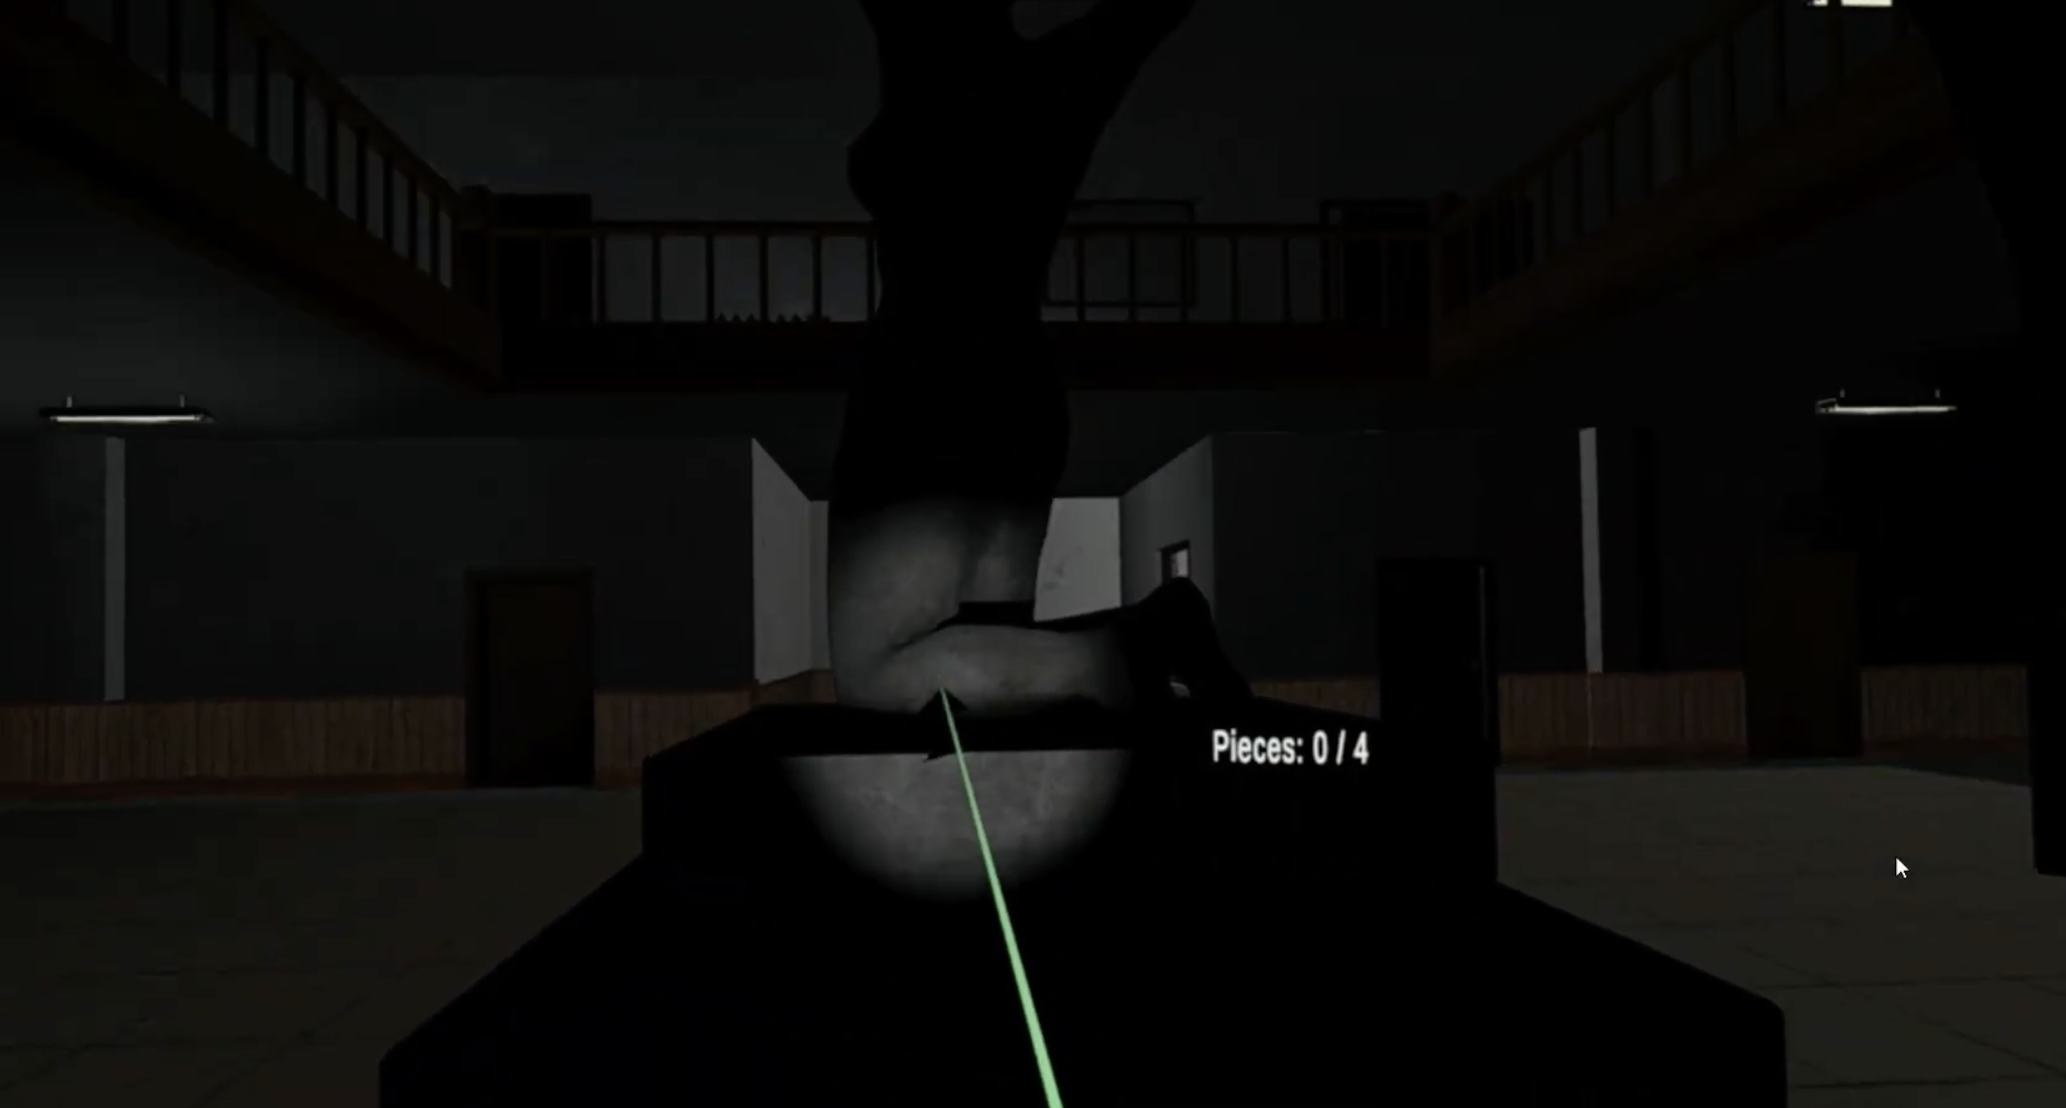
\includegraphics[width=0.45\linewidth]{phase2_map.png} &
    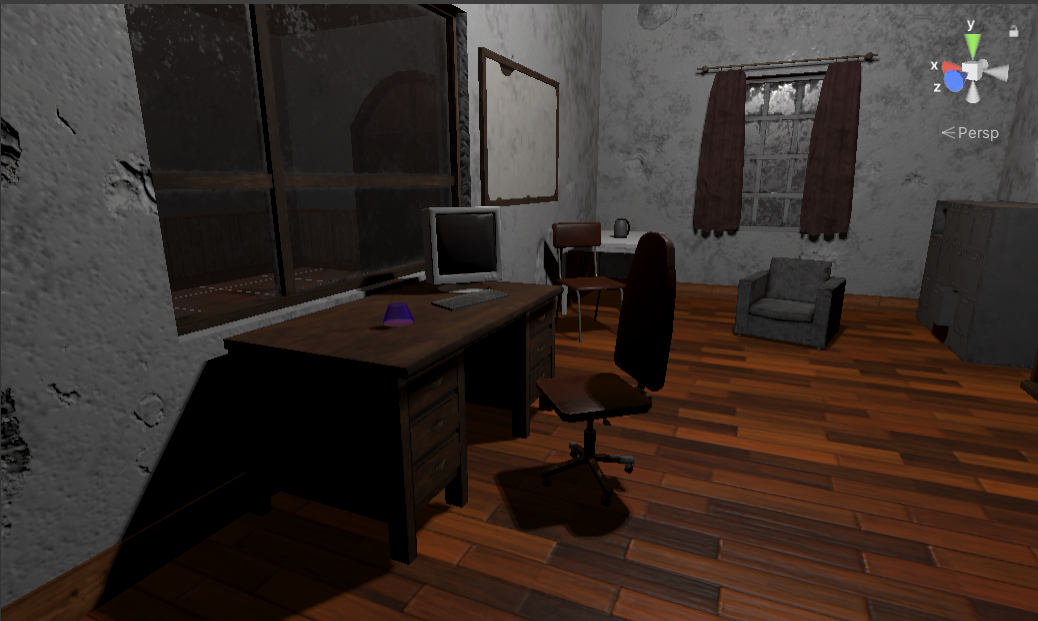
\includegraphics[width=0.45\linewidth]{phase2_item.png} \\
    (a) 屋敷内部の暗い環境 & (b) アイテム探索 (ビーカー収集)
  \end{tabular}
  \caption{Phase 2: 屋敷探索と予期不安}
  \label{fig:phase2}
\end{figure}

\subsubsection{Phase 3: ゾンビ追跡と驚き (Fear \& Surprise / Pursuit)}
\begin{itemize}
\item \textbf{目的}: 強い恐怖と特定対象に対する驚き反応を誘発する.
\item \textbf{メカニズム}: Phase 2と同一マップで敵(ゾンビ)追跡演出を活性化し即時的脅威刺激を提供することで, 高い覚醒と強い恐怖/驚き反応を誘導する. 知能型ゾンビAIがプレイヤーを追跡する(図 \ref{fig:phase3} (b)).ゾンビは一定距離内に接近すると停止して威嚇し(図 \ref{fig:phase3} (a)),再び接近を試みる2段階近接ロジック(\texttt{P3\_ZOMBIE\_NEAR\_1}, \texttt{P3\_ZOMBIE\_NEAR\_2})を持つ.
\item \textbf{終了条件}: プレイヤーが特定のドアを開けて脱出するか,ゾンビと一定回数接触すると \texttt{EXPERIMENT\_END} となり全データが保存される.
\end{itemize}

\begin{figure}[t]
  \centering
  \begin{tabular}{cc}
    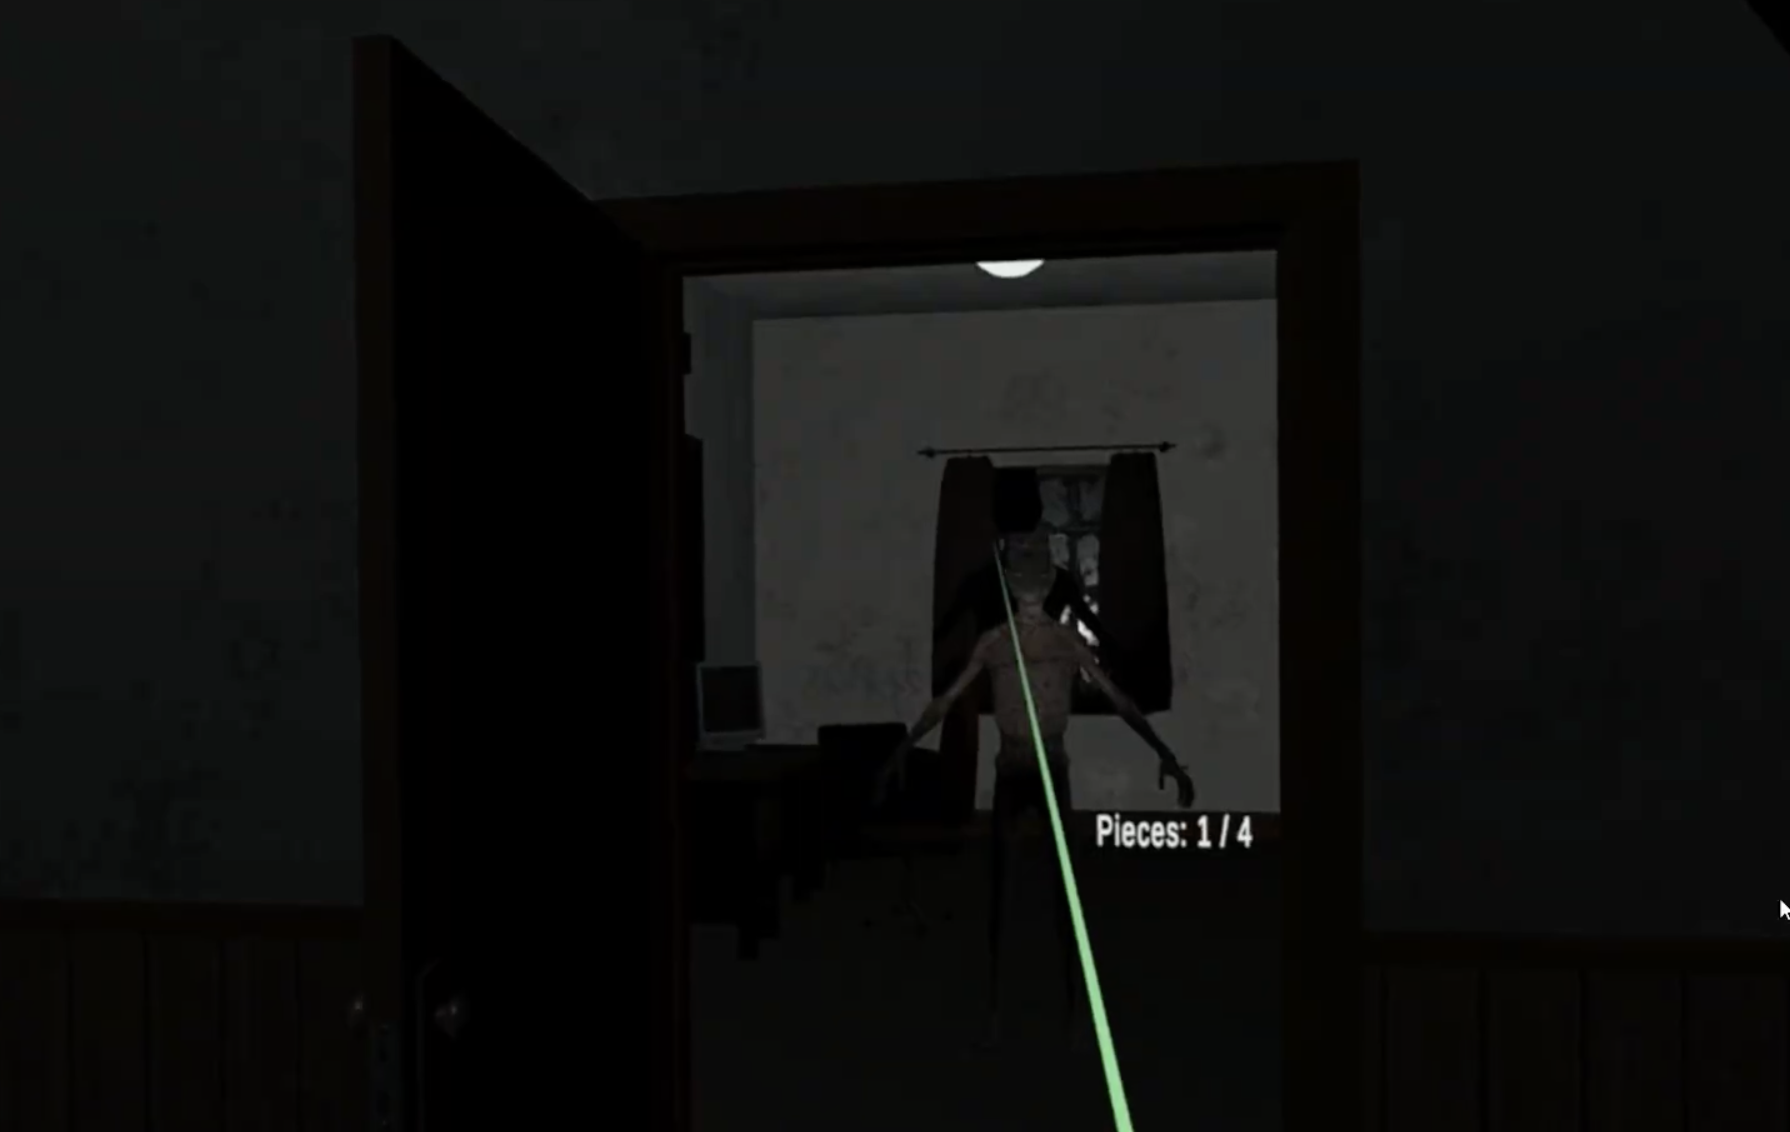
\includegraphics[width=0.45\linewidth]{phase2_zombie.png} &
    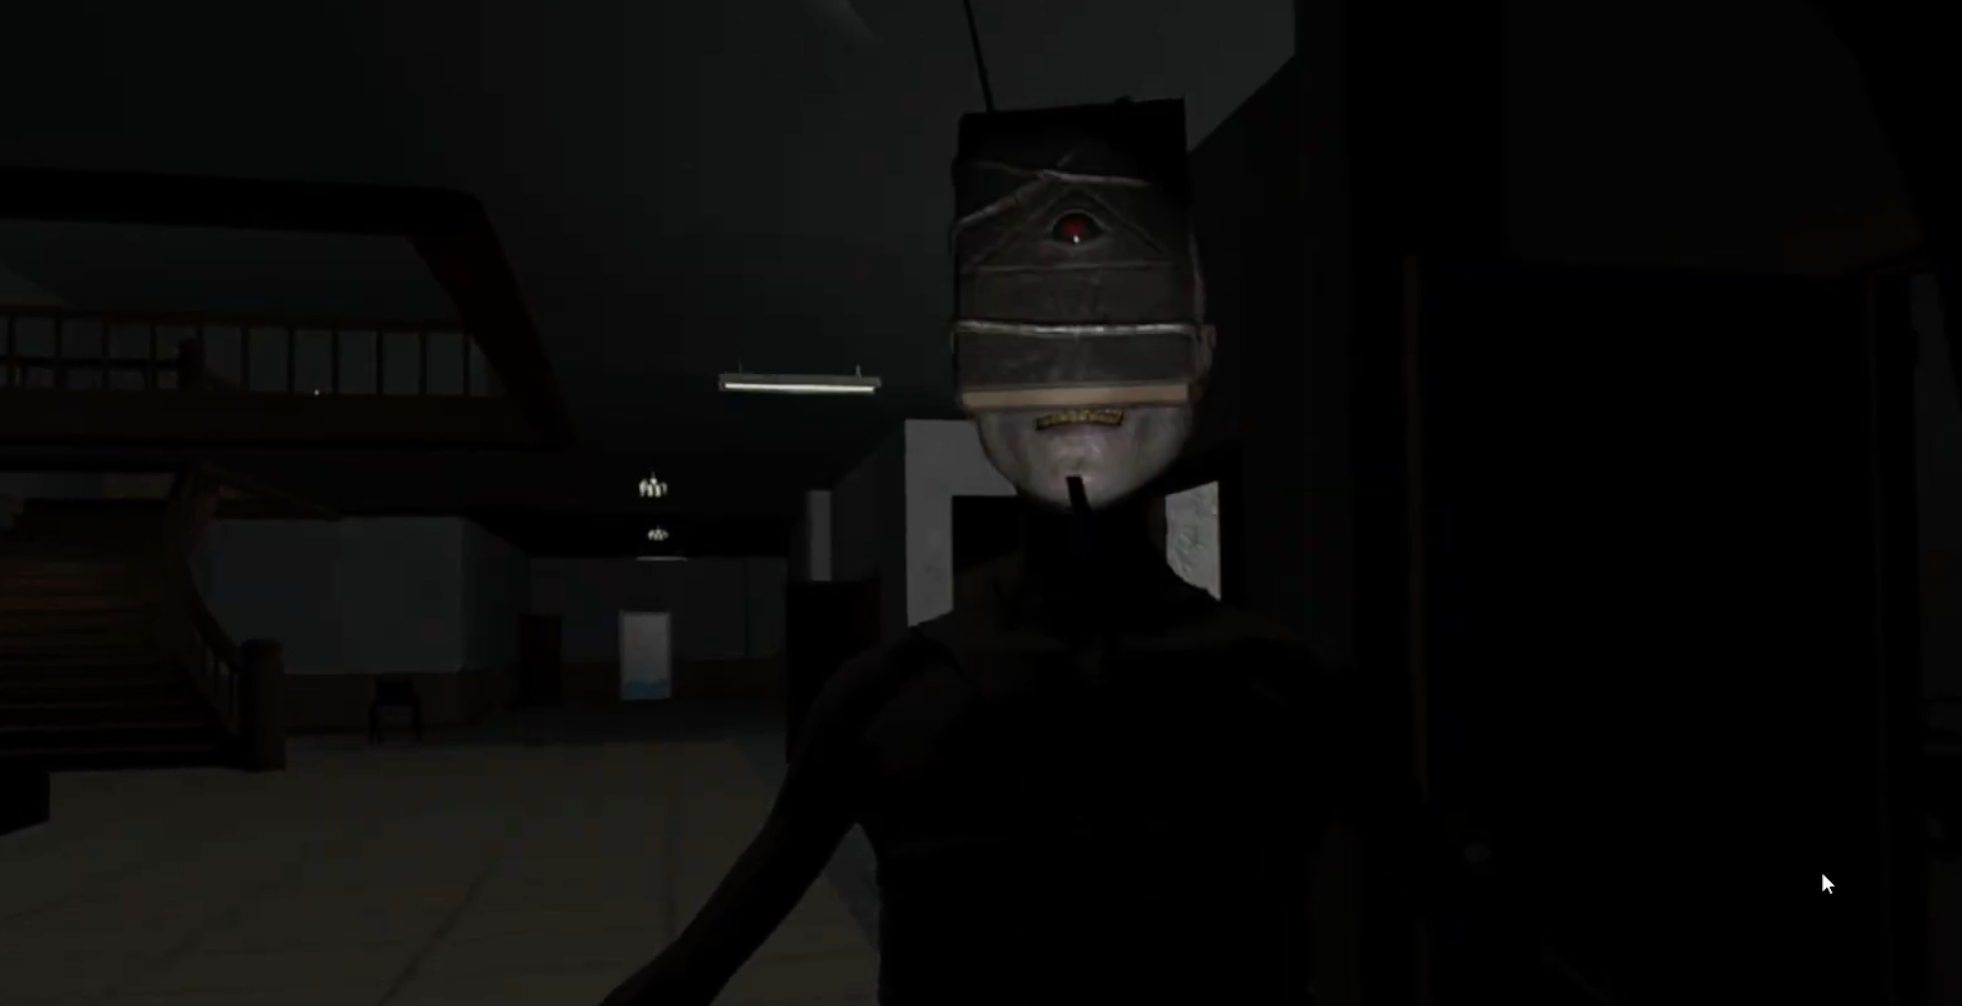
\includegraphics[width=0.45\linewidth]{phase3_trace.png} \\
    (a) 潜んでいるゾンビの発見 & (b) ゾンビによる追跡 (恐怖・驚き)
  \end{tabular}
  \caption{Phase 3: ゾンビ追跡と驚き}
  \label{fig:phase3}
\end{figure}




\chapter{実験}
本章では,提案したVR基盤マルチモーダル感情推定フレームワークを検証するために遂行した予備実験の設計と手順を提示する.
具体的に実験環境と装備構成,構成された刺激シナリオ,
データ収集および同期方式,そしてラベリング基準を順に説明する.


\section{実験設計および方法}

\subsection{実験目標}

本実験はUnityで開発したVRホラーコンテンツを通じて
ユーザの恐怖および驚き.そしてそれに伴う緊張や警戒の状態を段階的に誘導し,
提案した収集・同期システムを通じて生体信号および行動/イベント反応の変化を
捕捉できるか確認することに目的がある.
さらに収集されたマルチモーダルデータを活用して感情状態分類の可能性を初期評価し,
追加実験およびモデル改善点を導出する.
本研究の仮説は「VRコンテンツで誘発された恐怖/驚きおよび緊張状態は
生体信号(EDA,ECG,EMGなど)の有意な変化として現れ,
生体信号と行動/イベント情報を総合した特徴はユーザの感情状態を
区分するのに有用である」というものである.

\subsection{参加者}

予備実験には6名の被験者が参加した.
参加者は平均年齢28歳の健康な成人男性で,
VR使用経験があり心血管系または精神科的疾患がないと自己報告された.
すべての参加者は事前に実験手順と目的についての説明を聞いて同意書を作成し,
実験中いつでも中断を要請する権利があることを告知された.

\subsection{実験環境}

参加者はMeta Quest Pro HMDを装着し,
両手コントローラを使用して座った姿勢でVRコンテンツを体験した.
生体信号測定のためにBITalino(PLUX Biosignals)生体信号収集キットを使用した.



\subsection{刺激シナリオ}

VRコンテンツは「ランダム迷路型VRホラーゲーム」で構成され,
感情状態を段階的に誘導するためにPhase 0--3の順次構造で設計した.
Phase 0(安定)では刺激のない静的な環境で
安定した状態で60秒間維持を行い基準(baseline)生理値を確保する.
Phase 1(集中)では恐怖要素を排除した反応抑制課題(Go/No-Go)を遂行させ,
「集中」状態データを収集する.
Phase 2(恐怖/警戒)では暗い屋敷内部のマップを探索し
アイテムを収集するようにして不確実性と緊張を累積させ,
環境音,効果音,照明などの演出を通じて恐怖・警戒状態を誘導する.
Phase 3(恐怖・驚き強化)ではPhase 2と同一マップで
敵(ゾンビ)追跡演出を活性化し即時的脅威刺激を提供することで,
高い覚醒と強い恐怖/驚き反応を誘導する.
また,各フェーズおよびイベントの状況に応じて異なるBGMおよび効果音を使用した.
Phase 2の探索パートでは不気味で静かな環境音を再生し緊張感を高め,
アイテム獲得時には通知音を鳴らした.
Phase 3でゾンビが登場し追跡が始まると,テンポの速い緊迫した追跡用BGMに切り替えることで,
聴覚的刺激による恐怖と焦燥感を増幅させた.


\begin{table}[t]
  \caption{実験フェーズの構成と誘導される感情状態}
  \label{tab:experiment_phases}
  \centering
  \begin{tabular}{c|l|l|l|l}
    \hline
    \textbf{Phase} & \textbf{名称} & \textbf{環境および課題} & \textbf{誘導感情} & \textbf{予想される生体反応} \\
    \hline \hline
    0 & Baseline & 暗い部屋, 十字注視 (60秒) & 安定 (Rest) & ベースライン値の測定 \\
    \hline
    1 & Task & 明るい訓練室, Go/No-Go課題 & 集中 (Focus) & 認知負荷による軽微な上昇 \\
    \hline
    2 & Puzzle & 暗い屋敷, ビーカー(Piece)4個収集 & 不安/恐怖 (Fear) & 探索に伴うSCLの漸進的上昇 \\
    \hline
    3 & Chase & ゾンビ追跡, 脱出 & 恐怖/驚き (Panic) & HR, SCL, EMGの急激なピーク \\
    \hline
  \end{tabular}
\end{table}

\subsection{データ収集}

参加者がVRコンテンツを開始すると生体信号およびイベント/行動ログ収集が同時に開始される.
EDA,ECG,EMG信号はBITalinoを通じて1 kHzでサンプリングして収集する.
UnityアプリケーションはPhase開始/終了および主要イベント
(課題開始/反応,アイテム獲得,ゾンビ登場・近接,正面凝視など)を
イベントマーカーとして生成しTCPを通じてPython収集モジュールに転送し,
Pythonモジュールは生体信号ストリームを収集すると同時に
受信したイベントマーカーをログとして記録する.
コントローラ入力(ボタン/トリガー/スティック)およびHMD/コントローラ状態のような
VRインタラクション情報はUnityでタイムタグと共に記録した.
このようなデータは共通したPCシステム時間でタグ付けすることで同期し,
実験終了後Python基盤スクリプトを通じて一つの時系列データセットとして併合する.
全体VRプレイ時間は個人別に約7--10分が所要される.

\subsection{ラベリング}

収集された月経データには、システムが自動付与する「客観的ラベル」と、参加者の事後報告に基づく「主観的ラベル」を併用する.
まずPhase 0--3区間および主要イベントマーカー
(例：P1 trialオンセット,P2アイテム獲得,P3ゾンビ近接/正面凝視など)を基準に
前後一定時間(todo:具体的に何秒？)ウィンドウを定義して該当区間の正解ラベル候補として使用する.
その後,実験直後に参加者は事後アンケートを通じて
各Phaseおよび主要イベントで感じた感情強度
(例：恐怖,驚き,緊張,集中,没入など)を7点Likert尺度で評価する
(1：非常に低い,7：非常に高い).
自己報告スコアは正規化して区間ラベルの強度情報として活用し,
イベント基盤ラベルの妥当性点検および個人差分析に使用した.

\chapter{実験結果}

\section{主観的感情評価分析}
実験直後に実施したアンケート結果を分析し,参加者の主観的な感情変化を定量化した.この分析結果は生体信号解釈の基準点 (Ground Truth) として活用される.

\subsection{参加者別主観的恐怖度変化}
アンケートは7点リカート尺度 (1: 全く怖くない $\sim$ 7: 非常に怖い) を使用し,実験の進行順序 (探索 $\rightarrow$ ビーカー収集 $\rightarrow$ ゾンビ遭遇 $\rightarrow$ 追跡) に伴う感情変化を追跡した.

\begin{table}[t]
  \caption{実験後アンケート回答結果の要約}
  \label{tab:survey_results}
  \centering
  \begin{tabular}{c|c|c|c|c|c|c|l}
    \hline
    \textbf{ID} & \textbf{探索} & \textbf{収集} & \textbf{扉開放} & \textbf{追跡認知} & \textbf{追跡対峙} & \textbf{解放感} & \textbf{備考} \\
    & (Q2-1) & (Q2-3) & (Q2-6) & (Q3-1) & (Q3-2) & (Q3-3) & \\
    \hline \hline
    A & 2 & 3 & 5 & 6 & 3 & 5 & 後半恐怖上昇, 典型的パターン \\
    \hline
    B & 6 & 5 & 5 & 7 & 4 & 2 & 全体的に高い恐怖度, 周囲の騒音言及 \\
    \hline
    C & 4 & 4 & 6 & 6 & 7 & 6 & 一貫して高い恐怖および緊張維持 \\
    \hline
    D & 2 & 2 & 3 & 3 & 1 & 1 & 「ゾンビ追跡気づかず」, 低い恐怖度 \\
    \hline
    E & 5 & 6 & 6 & 6 & 7 & 7 & 非常に高い恐怖反応および解放感 \\
    \hline
    F & 3 & 5 & 6 & 1 & 1 & 6 & 「追跡認知できず」, 特異なパターン \\
    \hline
  \end{tabular}
\end{table}

\subsection{主観的反応の類型化}
アンケート結果に基づき,被験者を3つのタイプに分類することができる.

\paragraph{没入型恐怖反応群 (Immersion-Fear Group):}
参加者 A, B, C, E がこの群に該当する.彼らは実験設計の意図通り,Phaseが進行するにつれて (探索 $\rightarrow$ 追跡) 恐怖度が上昇する典型的なパターンを示した.特に参加者 C と E は追跡状況で最高点 (7点) を記録し,強いストレスを訴えた.

\paragraph{認知失敗群 (Cognitive Failure Group):}
参加者 D は「ゾンビが追いかけてきていることに気づかなかった」と明示的に回答した.この認知失敗により,追跡状況 (Q3-1) での恐怖度が3点と低く現れ,解放感 (Q3-3) もまた1点であり,実験終了に特段の感慨を感じていなかった.この結果はVRコンテンツにおける「注意集中」の失敗が感情誘発の失敗につながることを示している.

\paragraph{選択的認知群 (Selective Perception Group):}
参加者 F は探索および扉開放 (Q2-6) 段階では6点の高い緊張感を示したが,本来最も強烈な刺激である追跡段階 (Q3-1, 3-2) では「認知できなかった」として1点を記録した.しかし,解放感 (Q3-3) は6点と非常に高く,認知的には状況を逃したが,心理的には圧迫感を感じていた可能性を示唆する.

\chapter{考察}

\chapter{結論}

序論に対応させて結論を書く．結論を書く上での注意は以下の通りである．
\begin{itemize}
 \item まず本論文で何を提案し，何を実験し，何を明らかにしたのかを書く．
 \item やり残したことを「今後は，〜する」「今後の課題として〜が挙げられる」と書くと，
       「もう卒業するのにいつやるねん」ということになるので，今後の展望という形で書く．
 \item 序論では社会的な本研究の意義などを書いたはずなので，
       本研究を行ったことによって，どういう社会的な影響を与えることができるか，
       この研究が更に発展したものが社会に普及するとどのようなよいことがあるか，
       といった風呂敷を最後に大きく広げて終わる．
\end{itemize}

% 謝辞 %%%%%%%%%%%%%%%%%%%%%%%%%%%%%%%%%%%%%%%%%%%%%%%%%%%%%%%%%%%%%%%%%%%%%%%%%%%%%%%%%%

\acknowledgements

本研究を進めるにあたり...

% 参考文献 %%%%%%%%%%%%%%%%%%%%%%%%%%%%%%%%%%%%%%%%%%%%%%%%%%%%%%%%%%%%%%%%%%%%%%%%%%%%%%

\bibliography{reference}
\bibliographystyle{junsrt}



% 付録 %%%%%%%%%%%%%%%%%%%%%%%%%%%%%%%%%%%%%%%%%%%%%%%%%%%%%%%%%%%%%%%%%%%%%%%%%%%%%%%%%%

\appendix

\section{本文と直接関係ない知識}

付録は無いことが多いが，どうしても書いておきたいことは書いてもよい．
無い場合は，\verb|\appendix|からまとめて削除する．

% 研究業績

\papers %%%%%%%%%%%%%%%%%%%%%%%%%%%%%%%%%%%%%%%%%%%%%%%%%%%%%%%%%%%%%%%%%%%%%%%%%%%%%%

ここに，あれば自分の業績リスト．無ければ項目ごとコメントアウト．

\end{document}
